\chapter{Proposed Approach}
\label{chap:5_proposed_approach}

In this chapter, we present the methodology for solving the autonomous navigation task outlined in the previous chapter. Overall, we propose a CNN-MLP model where, given a depth image $\d_t$ and the quadrotor states $\s_t$, it decides a continuous velocity $\v^d_t$ and steering $r^d_t$ command that should avoid obstacles in a cluttered environment, while travelling towards some goal in 3-dimensional space.
We will present and discuss this two-part model's design choices, starting with the MLP module for learning the navigation policy, then later the encoder-decoder-based CNN inference network used for representation learning. An overview of the model is shown in \cref{fig:5_overview}.
\begin{figure}[hbt]
    \centering
    \makebox[\textwidth]{
        \hspace{15mm}
        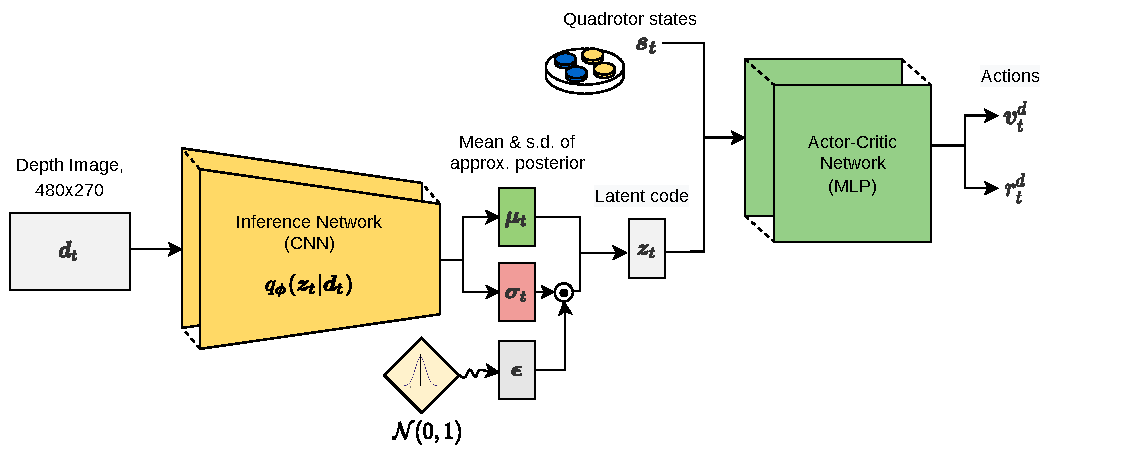
\includegraphics[width =1.1\textwidth]{figures/5_/5_overview.pdf}
    }
    \caption{An overview of our two-part model. The inference network (encoder) learns an approximate posterior distribution $\qzgived$, parametrised by a set of Gaussian distributions with an input-dependent mean $\boldsymbol{\mu}_t$ and diagonal covariance matrix $\boldsymbol{\sigma}_t$. We then sample this to get the latent representation $\z_t$. With $\s_t$ and $\z_t$, our agent -- a model-free actor-critic -- learns a policy $\actorpolicy$ which outputs a desired velocity $\v_t^d$ and yaw rate $r^d_t$.}
    \label{fig:5_overview}
\end{figure}

\section{Learning the Navigation Policy}
\label{sec:5_learning_navigation_policy}
Starting first with the navigation task, we solve the reinforcement learning problem through the use of PPO. Following the theory in \cref{subsec:2_PPO}, we aim to concurrently learn a critic value function $V_{\bt}(s)$ and actor policy $\pibtz$, parametrised with parameters $\bt$. To train our actor-critic for collision avoidance, we define a custom reward function and incorporate a \textit{curriculum} \cite{LearningWalkMassivelyParallel} during training.

\subsection{Reward Function}
\label{subsec:5_reward_function}
The reward function is one of the most powerful design tools within reinforcement learning. Using it to formalise the idea of a goal is also one of its most distinctive features \cite{suttonAndBartoBook}, since by deciding the reward structure of the environment, we can indirectly manipulate the learned agent behaviour to match the behaviour we hope to observe in testing. 
Though, for a navigational task, proper care must be taken to balance the rewards for different behaviours, such that an agent remains careful but also navigationally efficient. This is because the complex behaviour that an agent learns is based directly on the idea of maximising the total reward, which includes exploiting the environment and its reward function. Hence, any undesired behaviour that is observed in test-time is often a consequence of a poorly designed reward function.

By weighing these considerations, we construct a reward function that builds on the implementation in \cite{IsaacGym}, but with additional rewards $R$ and penalties $P$ to shape the agent behaviour for collision avoidance.
First, we motivate the agent to minimise its distance to goal by rewarding its inverse distance to goal:
\begin{equation}
    \rew{pos} \, (S_t) = \frac{\gain{pos}}{1 + ||\p_t||_2}
\end{equation}
Then, we define a set of desired behaviours we wish to see when the agent is close to goal: remain still $\rew{vel}$, stay upright $\rew{up}$ and do not spin $\rew{spin}$:
\begin{align*}
    \rew{vel} \, (S_t) &= \frac{\gain{vel}}{1 + ||\v_t||_2} \numberthis \\[2mm]
    \rew{up} \, (S_t) &= \frac{\gain{up}}{1 + \left|1 - \mathcal{I}_z(\q_t)\right|^2}\,, \qquad 
    \mathcal{I}_z(\q_t) = \frac{\epsilon_2}{\sqrt{1-\eta^2}} \numberthis\\[2mm]
    \rew{spin} \, (S_t) &= \frac{\gain{spin}}{1 + r^2} \numberthis 
\end{align*}
Here, we use $\mathcal{I}_z(\q_t)$ to denote the upwards-ness of the quadrotor, where the idea is to represent the quadrotor orientation $\q_t$ in axis-angle form and then find the normalised $z$-component of the axis. For $\rew{spin}$, $r$ denotes the quadrotor yaw rate as shown in \eqref{eq:4_quadrotor_states_detailed}.

As for the conservative behaviour, we specify three penalties terms: one for velocities in the blind directions of the quadrotor (vertical and backward) $\pen{vel}$, one for being too close to an obstacle $\pen{depth}$, and the last for collision $\pen{collision}$:
\begin{align}
    \pen{vel} \, (S_t) &=  \alpha_{\text{vert}} \cdot w^2 + \alpha_{\text{back}} \cdot v_{\text{back}}^2 \, \qquad v_{\text{back}} = 
    \begin{cases} 
      v & \text{if} \; v \leq 0 \\
      0 & \text{else} 
   \end{cases} \\[2mm]
   \pen{depth} (S_t) &= \mu_{\text{dist}} \cdot \max \, \big(0, d_{\epsilon} - d_\text{obst}(S_t)\big)^2 \\[2mm]
  \pen{collision} (S_t) &= \begin{cases}
     \gain{collision} & \text{if} \; d_\text{obst}(S_t) \leq d_\text{collision} \\
     \gain{collision} & \text{if contact force detected} \\
     0 & \text{else}
  \end{cases}
\end{align}
The depth penalty $\pen{depth}$ is a simple one-sided quadratic barrier function taken from \cite{collision_free_MPC}, consisting of a scaling parameter $\mu_{\text{dist}}$ and safety margin $d_\epsilon$. Intuitively, this means that quadrotor receives no penalty if it is further than $d_\epsilon$, but is penalised an obstacle within $d_\epsilon$ is in sight. Thus, this should motivate the agent to stop moving closer to an obstacle, and to turn elsewhere. Visually, the depth penalty is shown in \cref{fig:5_depth_penalty}.
\begin{figure}[hbt]
    \centering
    \hspace{2cm}
    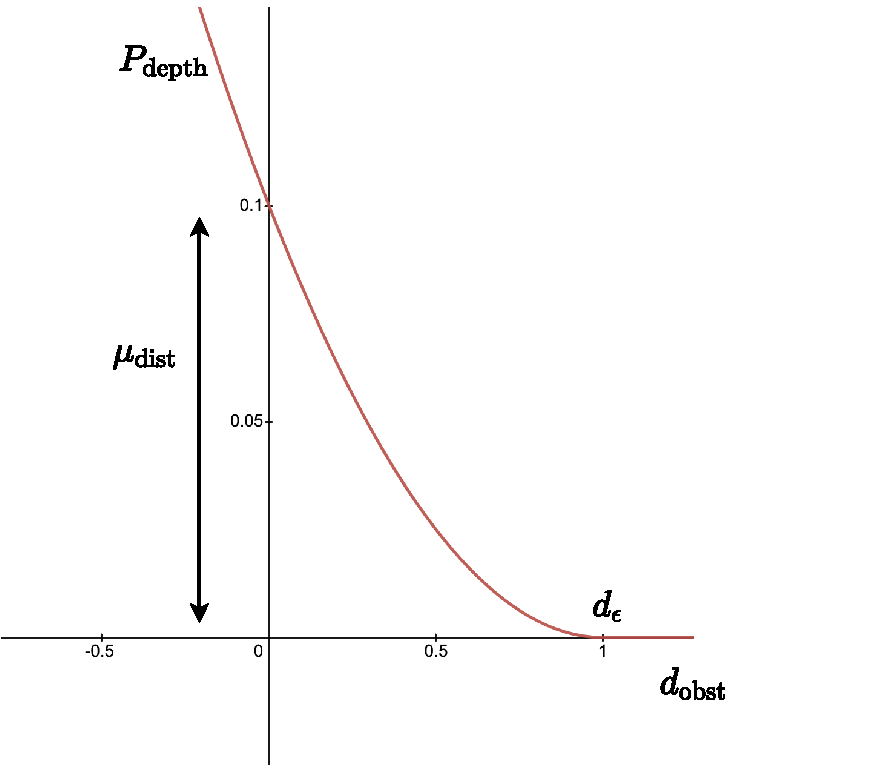
\includegraphics[width=0.6\textwidth]{figures/5_/5_depth_penalty.pdf}
    \caption{The depth penalty $\pen{depth}$ displaying the penalty for when an obstacle is closer than  $d_\epsilon = 1.0$m, when $\mu_{\text{dist}} = 0.1$. Diagram recreated from \cite{collision_free_MPC}.}
    \label{fig:5_depth_penalty}
\end{figure}

To find the distance to the closest obstacle $d_\text{obst}$, we project a point cloud from a depth image, and take the norm of each point in the point cloud with the camera position and finding the minimum. However, since we can only detect forward-facing collisions with the depth camera, we also detect collisions with a force sensor in simulation. 

From these, the full reward function is the sum of all rewards and penalties:
\begin{equation}
    R\,(S_t, \,A_t) = R_{\text{pos}} + R_{\text{pos}} \, (R_{\text{vel}} + R_{\text{up}} + R_{\text{spin}}) + P_{\text{vel}} + P_{\text{depth}} + P_{\text{collision}}
\end{equation}
where we specify $R_{\text{vel}}\,,\; R_{\text{up}}$ and $R_{\text{spin}}$ to only be important near goal by multiplying it with $\rew{pos}$.
Finally, the reward gains, penalty coefficients and distance parameters used for the reward function are listed in \cref{table:5_reward_parameters}.
\begin{table}[hbt]
    \centering
    \begin{tabular}{||c|c||}
    \hline
    \centering
        Reward Parameter & Value \\ \hline \hline
        $\gain{pos}$ & 2.0 \\  
        $\gain{vel}$ & 1.0 \\ 
        $\gain{up}$ & 1.0 \\ 
        $\gain{spin}$ & 1.0 \\ 
        $\gain{collision}$ & -2 \\
        $\alpha_{\text{vert}}$ & -0.1 \\ 
        $\alpha_{\text{back}}$ & -0.01 \\ 
        $\mu_{\text{dist}}$ & -0.1 \\ 
        $d_{\text{collision}}$ & 0.2 \\ \hline
    \end{tabular}
    \caption{List of reward gains, penalty coefficients and distance parameters used in the reward function.}
     \label{table:5_reward_parameters}
\end{table}

We note that each of the reward terms are at maximum when $\p_t, \v_t = \boldsymbol{0}$, $r = 0$ and the quadrotor is upright. At this point, the quadrotor is directly on the goal, with a reward of $R_t^\text{max} = \gain{pos} + \gain{pos}(\gain{vel} + \gain{up} + \gain{spin}) = 8$ at every timestep, assuming that we avoid all penalties. However, when the quadrotor is very far from goal, e.g. $>10$m, this goal-motivating reward begins to be very sparse. Combined with the conservative penalties, we can imagine that it will be difficult to train a policy end-to-end in a large cluttered environment due to negligible positive rewards for flying towards goal, and considerable negative rewards for going near obstacles.
This is also why we propose to use curriculum learning, which will be discussed in the next section.

\subsection{Curriculum Learning}
\label{subsec:5_curriculum}
The success of this thesis' approach can largely attributed to the setup and procedure for training the reinforcement learning agent.
The term \textit{curriculum} was introduced by \cite{LearningWalkMassivelyParallel} and is used to describe the idea of training a policy in levels of increasing difficulty. For collision free navigation, we leveraged this idea by training the quadrotor in progressively larger environments, with an increasing density of obstacles. The reason for this can be justified by two reasons: first, training a randomly initialised policy in a very difficult environment with sparse rewards can be extremely time consuming if not impossible; and second, collision avoidance is very generalisable -- once a quadrotor has learned to avoid one obstacle, it should not be difficult to extend this knowledge to two, and eventually many.

We assert that before a quadrotor can learn collision avoidance, it must first learn to fly towards the goal. Our primary concern is that reinforcement learning is generally considered sample-intensive, where learning a complicated policy may just come down to waiting for lucky sequence of actions to be repeatedly executed. In this thesis, we aim to minimise this ``luck factor'' and instead a propose a three-step process that should \textit{guarantee} successful training:
\begin{enumerate}
    \item First, learn to fly towards the goal with no obstacles present. 
    \item Then, learn basic obstacle avoidance by spawning the quadrotor and goal on opposite sides of \textit{one} obstacle, with the quadrotor facing the obstacle.
    \item Last, gradually increase the number of obstacles, the environment size and the episode length $T$ to obtain an advanced collision avoidance policy.
\end{enumerate}


\subsection{Network Architecture}
\label{subsec:5_MLP_architecture}
Moving on, the actor-critic network is chosen to be a shared three-layer MLP with two separate output heads: the policy head and the value function head.  Its architecture is shown in \cref{fig:5_actor_critic}. The policy $\actorpolicy$ is modelled by the actor network, which outputs a Gaussian distribution over actions for a given quadrotor state $\s_t$ and latent code $\z_t$. The value function is parametrised by the critic network that predicts the expected return (state value) for the same input.
\begin{figure}[hbt]
    \centering
    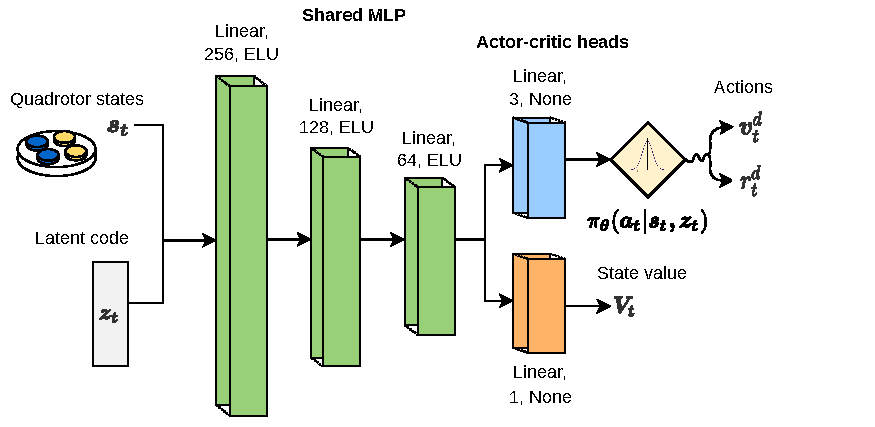
\includegraphics[width=0.9\textwidth]{figures/5_/5_actor_critic.pdf}
    \caption{The actor-critic network architecture. The actor and critic are parameterised by a shared base network comprised of a three-layer MLP with output dimensions $[256, 128, 64]$ and ELU activation functions, and two linear (fully-connected) output heads with linear activation functions. The actor parametrises a policy $\actorpolicy$ that outputs a Gaussian distribution over actions, while the critic parametrises a value function $\criticVF$ which predicts the expected return $V_t$.}
    \label{fig:5_actor_critic}
\end{figure}

\subsubsection{Shared Parameters in the Actor-Critic}
The concept behind using a shared structure in the actor-critic networks is that the \textit{base network} learns the \textit{features} our input, so that these can be used by the \textit{network heads} for \textit{task-specific prediction or classification}. Essentially, it is the same as representation learning, where the last layer of the shared MLP is contains the representation or features of the input. 
We can assume that in order to produce a correct velocity and yaw rate reference, the model should have some understanding of the agent relative its surroundings. Though in a similar vein, to be able to predict the expected return for a particular state requires the same understanding. So, in general, if two output tasks are largely related, but utilise the same input, it makes sense to have a shared parametrisation for the base network, with two task-specific heads.

\subsubsection{Size of the Network}
The size of the network was largely chosen according to other baseline models in \cite{IsaacGym} and from previous experience from the project thesis \cite{project_thesis}. From \cite{IsaacGym}, we noted that many examples utilise much larger networks but these were also applied to tasks with ``more difficult'' observation-action mappings \cite{shadowHand, AMPMotionPriors} -- in essence just having a much higher dimensional observation and action space.
This idea of using larger networks is that they have a larger \textit{generalisation potential}, thus enabling them to do well in more complicated tasks. Moreover, recent research also states that overparametrisation of neural networks might even be necessary to have robust results \cite{bubeck2021aLawOfRobustness}.
However, from experience in the project thesis, we found that larger networks take longer to train and do not necessarily produce better results immediately, therefore motivating a more conservative approach which is more in line with machine learning teachings: starting simple and increasing the complexity underway. From this, we found that a base network with size [256, 128, 64] was reasonable, along with 64 neurons for each head.

\subsubsection{Activation Functions}
In \cref{fig:5_actor_critic}, we note the use of two types of activation functions, the exponential linear unit (ELU) and linear (None), where most noteworthy is the choice of the linear activation function for the final network layer. Traditionally, we choose the final activation function based on the type of problem we have -- like \textit{sigmoid} for logistic regression (prediction or binomial classification tasks), or \textit{softmax} for multinomial logistic regression (multi-class classification). For continuous control problems with normalised actions spaces, we often wish to limit our actions to a range of $[-1, 1]$, which actually makes \textit{tanh} the most suitable activation function. Nevertheless, the decision to use the linear activation function was largely as a result of the baseline implementations in \cite{IsaacGym}. Instead, as an implementation detail, actions were left unbounded from the network but were clipped if their values exceeded $[-1, 1]$. 

Next, the exponential linear unit \cite{ELU} was also used due to being the default implementation in \cite{IsaacGym} -- with it also being used to solve other difficult tasks \cite{shadowHand, LearningWalkMassivelyParallel}. An alternative for MLPs is of course the widely popular rectified linear unit (ReLU) \cite{ReLU}, but the ELU differs slightly as it has negative values for inputs less than zero. This is shown more clearly in \eqref{eq:5_elu_activation} and \cref{fig:5_relu_elu}.
\begin{align}
        f_\text{ELU}(x) &= \begin{cases}
          x & \text{if} \; x > 0 \\
          \alpha \, (\exp{(x)} - 1) & \text{if} \; x \leq 0
        \end{cases}, \label{eq:5_elu_activation} \\
        f_\text{ReLU}(x) &= \begin{cases}
          x & \text{if} \; x > 0 \\
          0 & \text{if} \; x \leq 0
        \end{cases} \label{eq:5_relu_activation}
\end{align}
\begin{figure}[hbt]
    \centering
    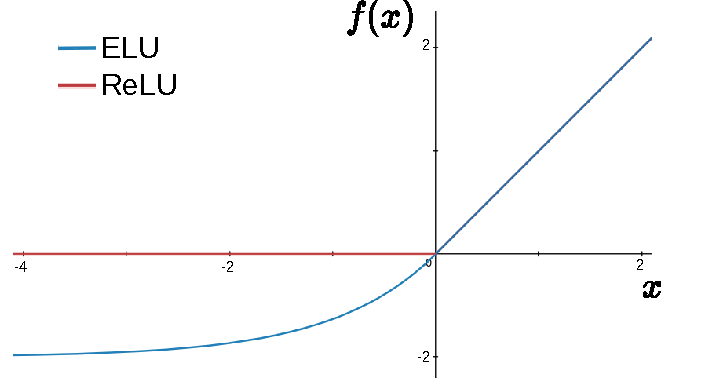
\includegraphics[width=0.5\textwidth]{figures/5_/5_relu_elu.pdf}
    \caption{Visualising the difference between the exponential linear unit (ELU) (with $\alpha = 1$) and rectified linear unit (ReLU) activation functions.}
    \label{fig:5_relu_elu}
\end{figure}

The primary reason for using ELU rather than ReLU is that one of the most significant problems of ReLU is that of \textit{dead neurons}. This problem occurs when a neuron is pushed to a negative weight (e.g. from a large update), because the gradient of the ReLU activation (its output) w.r.t the negative neuron weight will always be zero. To illustrate clearly, consider the perceptron $y = \text{ReLU}(Wx + b)$. When the a \textit{positive input} $x$ is multiplied with \textit{negative weights} $W$, the output $y$ is zero, and so too the gradient $\frac{\delta y}{\delta W}$. 
Conversely, if the \textit{input} $x$ and weights $W$ are \textit{negative}, the output $y$ is non-negative but the gradient of the output w.r.t the weights $\frac{\delta y}{\delta W} = \text{ReLU}' (x)$ is still zero because the ReLU gradient $\text{ReLU}'$ is zero for negative inputs.
As a result, the network weight will never be able to update itself as the gradient will be zero indefinitely, irrespective of the input data.
The benefit of ELU is that its gradient is non-zero for negative inputs close to zero. This helps to solve the \textit{dead-neuron problem} as it produces non-zero gradients that helps to nudge network weights in the right direction, despite them having negative inputs. \todo{maybe move to theory}

However, it can be argued that having some sparsity in the network (due to dead neurons) is actually an advantage, which is why ReLU is the default recommendation by \cite{DeepLearningBook} for modern neural networks, and is also used in \cite{AMPMotionPriors} for its actor-critic MLP. Then again, too much sparsity can result in the network losing some of its generalisation capacity.

\section{Learning the Depth Representation}
\label{sec:5_learning_representation}
To tackle the unsupervised representation learning problem, we use a convolutional VAE to learn the latent representation for the depth data $\d$. We use the method presented by \cite{variational_bayes} for optimising the VAE, whose theory is outlined in \cref{subsec:2_VAE_variational_autoencoders}. Additionally, to both deal with the constrained dimension of the latent space and make our VAE suitable for collision avoidance, we introduce a custom loss function that allows us to specify which depth characteristics the VAE should prioritise in its reconstructions, and choose a lightweight network architecture inspired from \cite{deepCollisionPredictorOracle} and \cite{vae_decoder_architecture}.

\subsection{Ideal Depth Reconstruction With a Customised Reconstruction Loss}
We first recall that the \textit{reconstruction loss} in \eqref{eq:2_vae_loss_estimator_single_datapoint} defines the learned behaviour of our generative network $\pdgivez$. In a vanilla VAE, it defines that the decoder $\pdgivez$ should learn to reconstruct $\d_t$ from $\z_t$, where $\z_t$ is the sampled latent code from our encoder $\qzgived$ for a given $\d_t$. Now, the key insight is that in order to properly reconstruct $\d_t$, any features of $\d_t$ that should be reconstructed must be present in $\z_t$ -- from which the VAE learned to do through the joint optimisation of the encoder and decoder in \eqref{eq:2_vae_loss_estimator_dataset}.
This implies that if we define certain features of $\d_t$ to be more costly than others, their loss will be over-represented in the reconstruction loss, and the VAE would prioritise learning these in its latent space so that these specific features could be reconstructed, and the VAE loss minimised. 

Thus, our approach is to \textit{alter the reconstruction loss} such that the VAE learns which features of the depth image distribution to prioritise in its latent space. With this, we attempt to prioritise the features in \cref{sec:4_representation_learning_task} in the latent space by presenting the following modifications:
\begin{enumerate}
    \item \textbf{Filtered targets} -- Instead of using the input $\d_t$ as the target reconstructions of our generative model $\pdgivez$, we use a filtered depth image $\d^f$ as the target. This means that for a given depth image $\d_t$, the generative network instead learns a probability distribution $\pdfgivezt$, where $\d^f_t = f(\d_t)$ is given by a deterministic filtering process $f$ of the depth image $\d_t$, and $\z_t \sim \qzgived$ is the sampled latent code from our encoder with input $\d_t$.
    \item \textbf{Depth weighting} -- We weigh the pixel-wise reconstruction error by a function of its observed depth. This means that the reconstruction error for pixels showing close obstacles in $\d^f_t$ are weighed more than pixels of far obstacles.
    \item \textbf{Added edge loss} -- We add the an additional mean-absolute error (MAE) term to the reconstruction error of filtered-obstacle edge pixels.
\end{enumerate}

To go more in detail, the filtering process is the IP-Basic algorithm \cite{filtering_depth_completion} for dilation and hole closing, as used in \cite{LearningStateRepresentation} and \cite{deepCollisionPredictorOracle}. Its implementation is a result of a few benefits for our task. First, minimising the complexity of depth images by rounding shapes emphasises only learning rough shapes. Also, as dilation increases obstacle sizes, filtering provides an extra layer of safety regarding collision avoidance. Finally, filtering also removes noise, which can be important when testing this framework on a real robotic system.
Then, to avoid the extra computational load of pre-filtering depth images on the robot, we use filtered images as reconstruction targets for some depth input, such that the VAE learns to implicitly perform the filtering process in its forward-pass \cite{LearningStateRepresentation}.

As for the depth weighting, we multiply the pixel-wise error of a reconstruction with the bounded depth gain $K_{\text{depth}}(d_{i,j})$, a function of the filtered-depth pixel value $d_{i,j}$:
\begin{equation}
    K_{\text{depth}}(d_{i,j}) = \alpha_\text{depth} \cdot \min \Bigg(\frac{1}{d_{i,j} + 0.5}, 1\Bigg) \qquad \text{for} \quad  i, j \in \dim \, (\d_t^f)
\end{equation}
which is illustrated in \cref{fig:5_depth_gain}.
\begin{figure}[hbt]
    \centering
    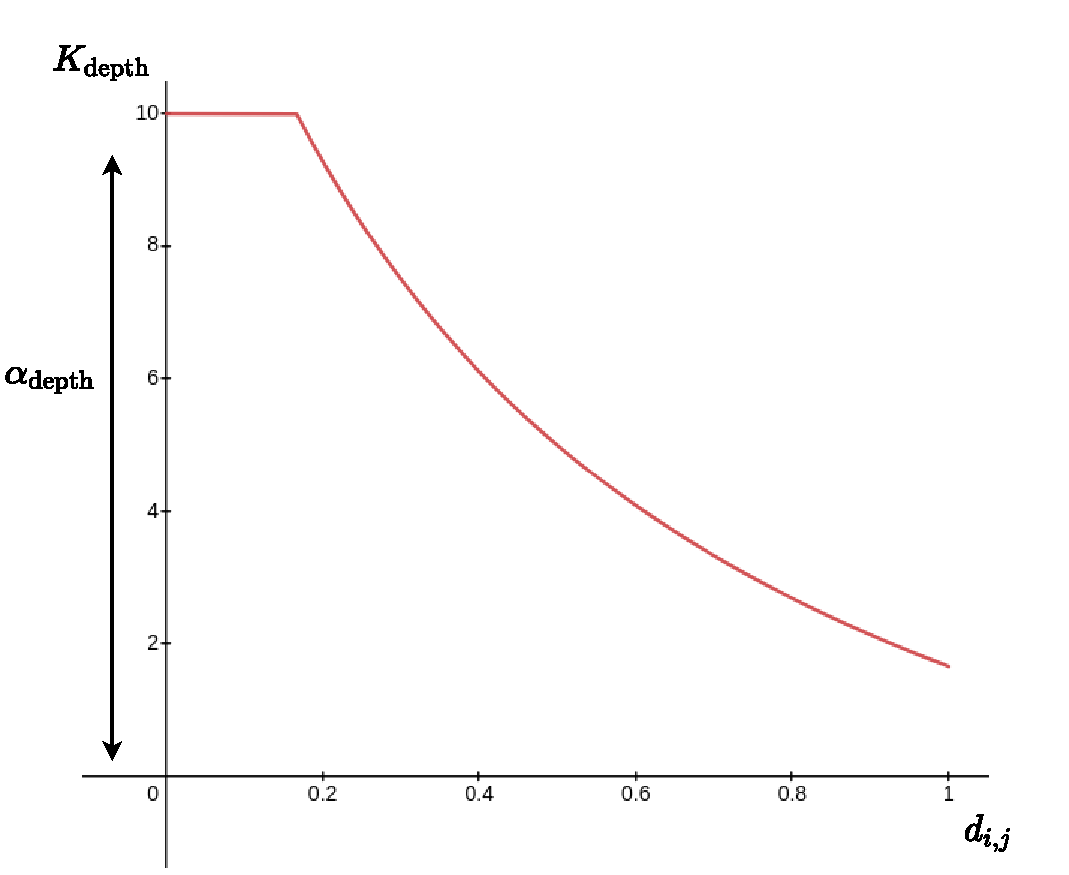
\includegraphics[width=0.5\textwidth]{figures/5_/5_depth_gain.pdf}
    \caption{The depth gain to weigh the pixel-wise reconstruction error. Reconstruction errors for very close obstacles (pixel values $d_{i,j}<0.16$) are weighed the same, with $\alpha_\text{depth} = 10.0$.}
    \label{fig:5_depth_gain}
\end{figure}
The idea for the depth weighting is that if we increase the reconstruction error according to its closeness, the pixel-wise loss of close obstacles should dominate the pixel-wise loss of obstacles far away. So close obstacles should be prioritised in the latent space representation.
Intuitively, this is particularly important for collision avoidance: we wish to distinguish between pixel-wise errors for obstacles far away compared to those immediately nearby. For example, a 1m error for an obstacle 7m away should be considered less important than the same as a 1m error for an obstacle 1.5m away.

We also see that thin obstacles are expected to be reconstructed when they are close by combining depth weighting with filtered targets. This is because their reconstruction targets are more prominent, as many more pixels will produce a high loss, particularly at close range.

Finally, we used a simple homemade procedure to implement the added edge loss. First, we used a Canny edge detector \cite{canny_edge_detection} to find the obstacle edges in $\d_t^f$. After, we used a Gaussian filter to dilate the edges -- taking any pixel-value over 0 as an edge. Finally, the pixel-wise MAE of filtered depth reconstruction was multiplied by this image-edge mask to achieve the edge loss. Since we motivated this for clearer reconstructions, the Gaussian filter had to be used to dilate the edges of the image-edge mask. This is because, for the MAE loss to account for the object's shape, it is essential to add the pixel-wise error along the edges of obstacles and the pixel-wise error of neighbouring pixels. 


\subsection{Network Architecture}
\label{subsec:5_vae_architecture}
With the loss function covered, what remains is the architecture of the VAE. As mentioned, our VAE design was mainly inspired by the work of \cite{deepCollisionPredictorOracle} and \cite{vae_decoder_architecture}, where we utilise a convolution-based encoder-decoder structure.
The overall structure of the VAE is shown in \cref{fig:5_vae} and its parameters are detailed in \cref{app:vae_params}.
\begin{figure}[hbt]
    \centering
    \makebox[\textwidth]{
        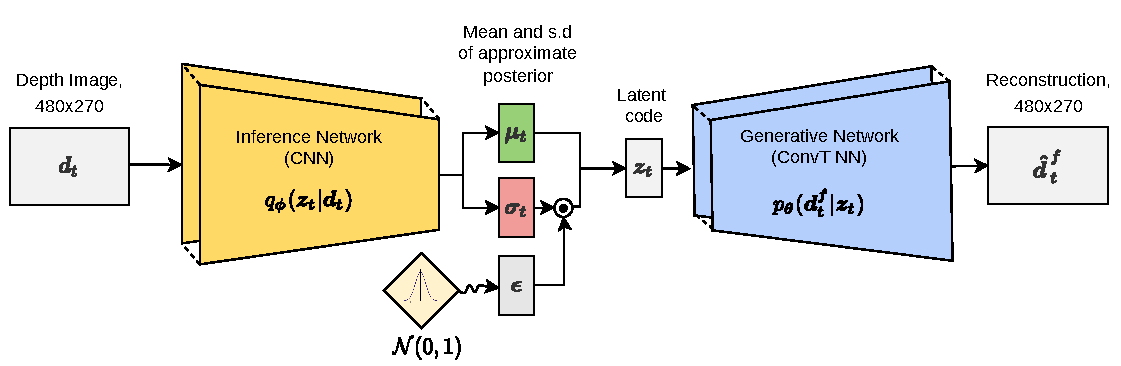
\includegraphics[width=\textwidth]{figures/5_/5_vae.pdf}}
    \caption{The VAE network architecture. The encoder is parametrised by a CNN, while the encoder is parametrised by a transposed CNN (ConvT NN). Given a depth image $\d_t$, we can sample from the inference network $\qzgived$ to obtain a latent code $\z_t$. The generative network $\pdfgivez$ then learns to construct the filtered depth image $\d^f_t = f(\d_t)$ from the latent code$\z_t$.}
    \label{fig:5_vae}
\end{figure}

\subsubsection{Inference Network}
\label{subsubsec:5_vae_inference_network}
Our encoder is follows the CNN design of \cite{deepCollisionPredictorOracle}, though utilises instead two convolution layers before a ResNet8 \cite{KaimingResNet}, with two fully-connected layers at the end. Its structure is shown in \cref{fig:5_encoder}, while the residual blocks are depicted in \cref{fig:5_res_block}.
\begin{figure}[H]
    \centering
        \makebox[\textwidth]{
        \hspace{1mm}
        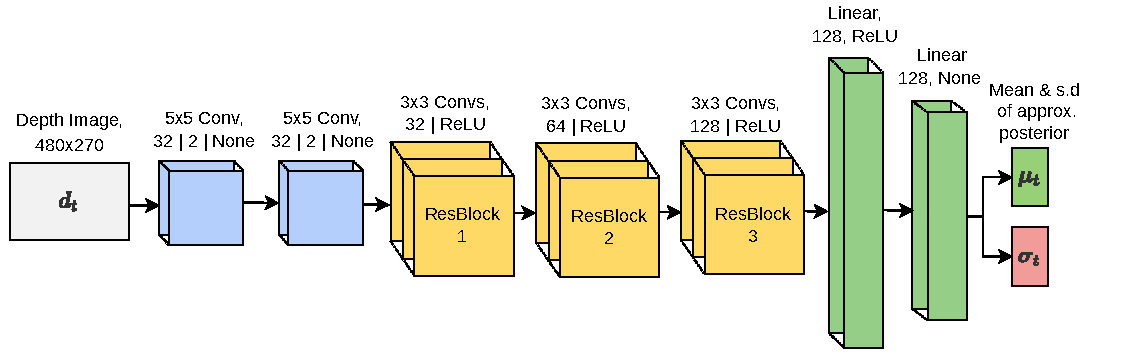
\includegraphics[width=1.\textwidth]{figures/5_/5_encoder.pdf}
    }
    \caption{The encoder network architecture. It comprises of two convolution layers, with 32 $5\times5$ filters with stride of 2, three residual blocks with $[32, 64, 128]$ output filters, and two fully connected layers with output dimensions $[128, 128]$. The dimension of the feature map is (roughly) halved for each convolution layer and residual block, due to the 2-strided convolutions. The size of the feature map at after the last convolution is $15\times9$. (See \cref{app:vae_encoder} for details)}
    \label{fig:5_encoder}
\end{figure}
\begin{figure}[H]
    \centering
    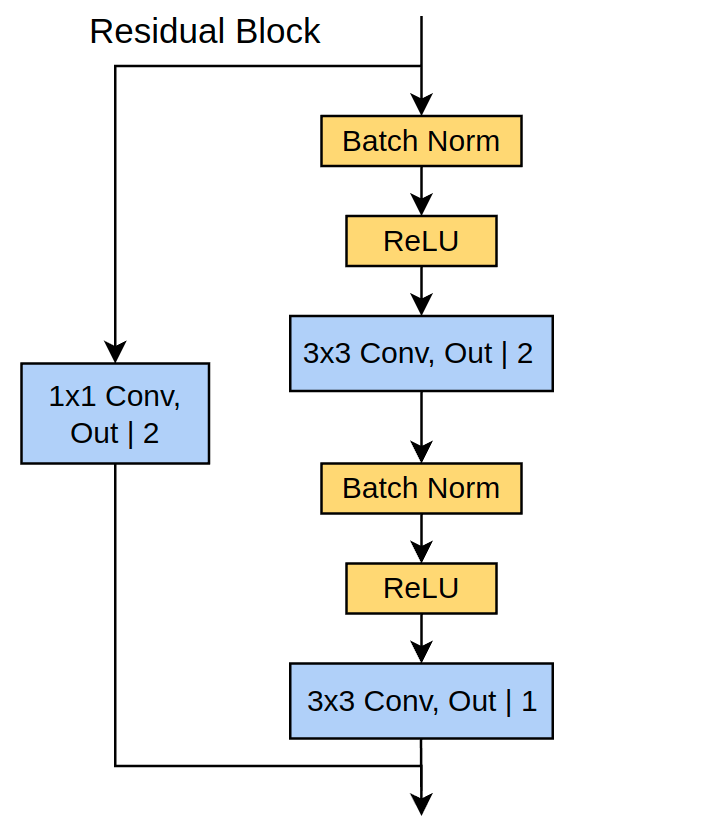
\includegraphics[width=0.4\textwidth]{figures/5_/5_res_block.png}
    \caption{The residual block architecture. A convolution by a $1\times1$ filter (kernel), with stride 2 is applied to the shortcut connection. $Out$ represents the number of filters of the residual block.}
    \label{fig:5_res_block}
\end{figure}
Regarding our design choices, these were primarily motivated by two factors -- we desired a lightweight network and wished to reduce the dimension of the feature map to be small enough but not too small. 
The ResNet8 was suitable to satisfy the first aspect, while the depth of the network (through strided convolutions) was decided to satisfy the other. We also found during testing that reducing the feature dimension below $15 \times 9$ (to $8 \times 5$) resulted in a much worse reconstruction output, discouraging the use of another residual block or strided convolution layer.
However, this choice resulted in a dramatically sized linear layer that accounted for 86\% of the encoder weights -- ($128 \cdot 15\times9) \cdot 128$ connections.
Nevertheless, this was unavoidable since 128 was the minimum number of neurons in the linear layer (64 means and log-variances), which left the alternatives: to either reduce the feature dimension or the number of filters. Though, both options were tested and did not improve results, leaving the conclusion that this is a feature and not a disadvantage of our encoder.


\subsubsection{Generative Network}
\label{subsubsec:5_vae_generative_network}
The generative network is inspired from \cite{vae_decoder_architecture}, with an additional linear layer and transposed convolution layer. Its architecture is shown in \cref{fig:5_decoder}. 
\begin{figure}[hbt]
    \centering
        \makebox[\textwidth]{
        \hspace{1mm}
        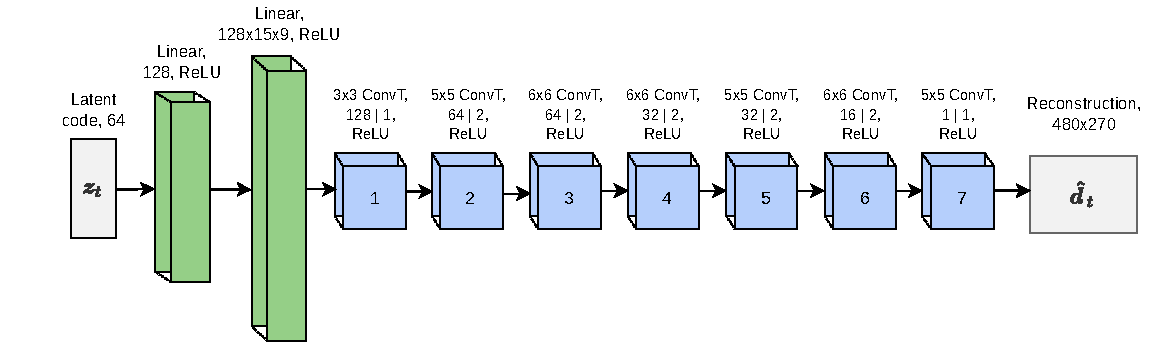
\includegraphics[width=\textwidth]{figures/5_/5_decoder.pdf}
    }
    \caption{The decoder network architecture comprises of two linear layers and seven transposed convolution layers. Each strided transposed convolution roughly the dimension of the feature map, to achieve the final dimension feature map dimension $480\times270$. (See \cref{app:vae_decoder} for details)}
    \label{fig:5_decoder}
\end{figure}
The primary design rule for autoencoders is that the decoder should be a mirror of the encoder, so that the network resembles an \textit{hourglass}. As a result, we followed the encoder with two linear layers, including the large linear layer that connects 128 neurons to 128, $9\times5$ filters. As for the transposed convolutions, this is relatively simple but effective design. The only design choice here was the filter size and number of filters, though these were chosen primarily to match the layer-wise feature dimensions of the encoder and their overall sizes.

Vigorous testing was also done with a ResNet8 decoder, which was designed to mirror our encoder. However, despite its more advanced structure -- with batch normalisation and shortcut connections -- no significant performance gain was observed in training. Conversely, divergence in training was often observed when training on the whole dataset, for unknown reasons. Therefore, a final decision was made to use the decoder in \cref{fig:5_decoder}.